\chapter{System Overview}
This chapter provides a high level overview of the hexapod, starting with the hardware, then the software, and finally the simulation
environment.
\section{Hardware}
The physical hexapod is primarily the same hexapod described in \cite{erasmus2023guidance}, this robot is shown in figure \ref{fig:hexapod}. For computation, a JetsonNano and Teensy2.0 \ac{mcu} is used. Actuation of the six, three degrees of freedom, legs is handled by 24 Dynamixel RX-64 servos. Sensing is handled by a Realsense D435i \ac{rgbd} camera, which includes a \ac{imu} (However the \ac{imu} is not utilised in this project.) Two Marvelmind ultrasonic \ac{lps} beacons are also present on the robot, although these are not used either.
\begin{figure}[h]
    \centering
    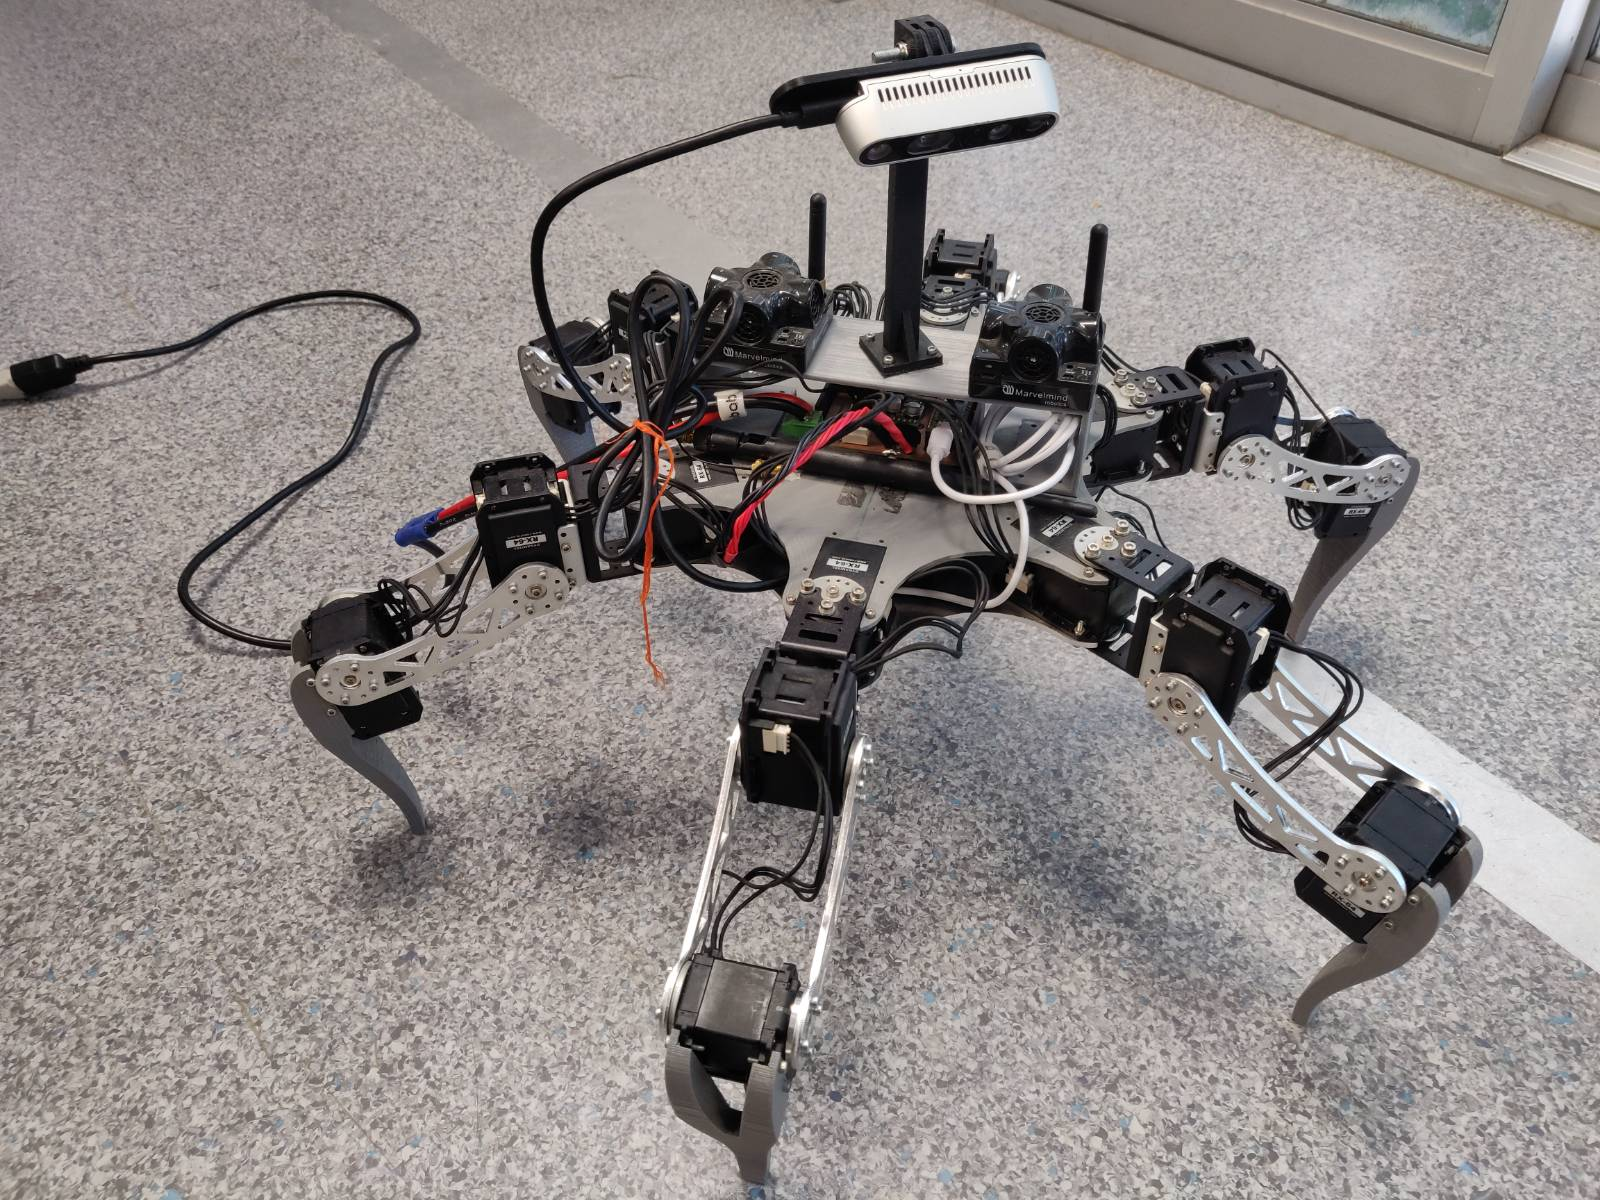
\includegraphics[height=6.6cm]{hexapod.png}
    \caption{Physical Hexapod}
    \label{fig:hexapod}
\end{figure}

\noindent
The only alterations made from the version describe in \cite{erasmus2023guidance} is the thickening of the wires powering the JetsonNano,
to prevent a voltage drop, and the replacement of the 3D printed legs with laser-cut aluminium legs, to prevent leg flexure.

A power cable is shown running to the left and going off image. All tests were conducted using 14.8V
from a bench power supply plugged into the battery port. This was done for convenience and can easily be swapped for a battery.

\section{Software}
The most basic software flow for a robot walking over flat terrain is shown in figure \ref{fig:basic_sys}. This system does not sense
its environment in any way and simply moves its feet along predetermined paths.
\begin{figure}[h]
    \centering
    % \hspace{-1.38cm}
    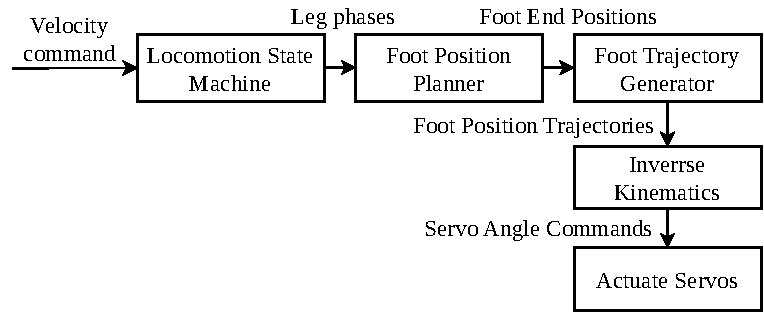
\includegraphics{Diagrams-SysDiffBlockBefore.drawio.pdf}
    \caption{Basic system operation}
    \label{fig:basic_sys}
\end{figure}

\noindent
This basic system will work well enough for walking over flat terrain, but will struggle once any
deviation in terrain height is present. Thus, the proposed, more advanced system, operates with the flow shown in figure \ref{fig:adv_sys}.

The advanced system uses similar components as the basic system, but with the foot end position planner modified to incorporate
checks against a score map and a height map to validate, and if necessary, adjust the foot 
end positions to place the feet at suitable positions in the  terrain. If no suitable adjusted foot positions and trajectories
can be found given the terrain, then the hexapod does not execute the motion and freezes in place. The human operator or
high-level guidance system must then change the overall path of the hexapod. However, this is outside the scope of the current
project.

\newpage
\begin{figure}[h]
    \centering
    % \hspace{-1.38cm}
    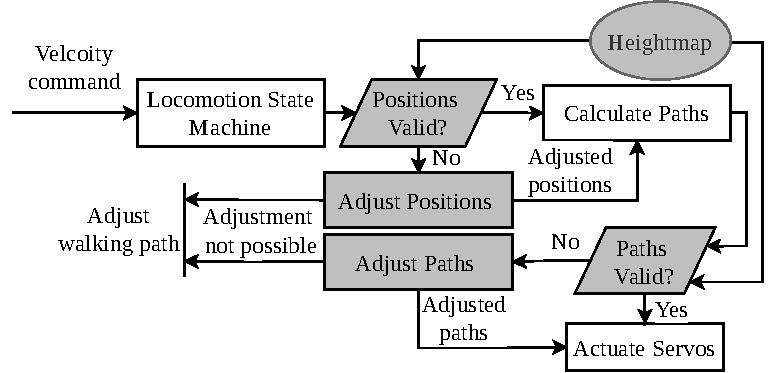
\includegraphics{Diagrams-SysDiffBlockAfter.drawio.pdf}
    \caption{Advanced system operation}
    \label{fig:adv_sys}
\end{figure}

\noindent
The goal of maneuvering uneven terrain is achieved by a combination of 4 primary systems, namely a mapping, 
foot placement optimisation, motion control and a localisation system. A high-level overview of the system implementation can be seen
in figure \ref{fig:system_diagram}.
\begin{figure}[h]
    \centering
    % \hspace{-1.38cm}
    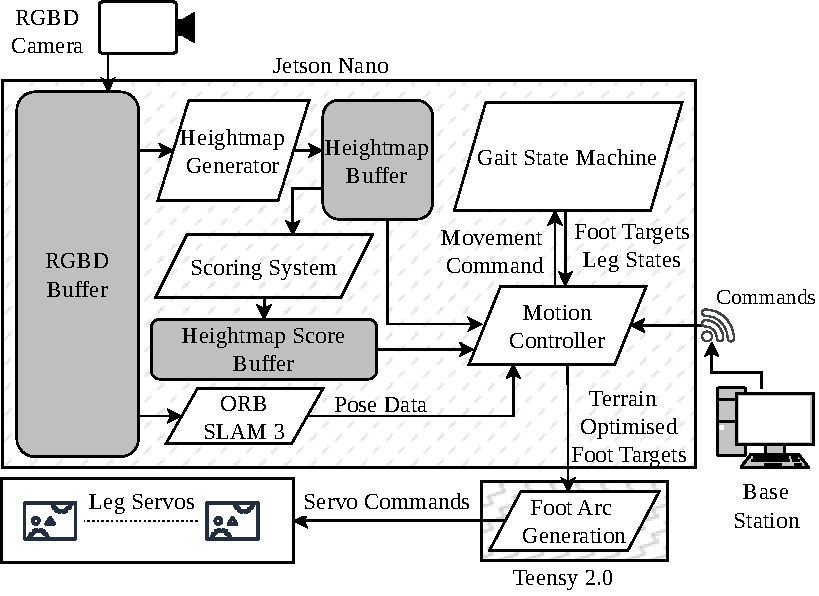
\includegraphics[width=0.93\textwidth]{HexapodSystemDiagram.drawio.pdf}
    \caption{Physical system diagram}
    \label{fig:system_diagram}
\end{figure}

\noindent
The mapping system utilises the \ac*{rgbd} camera to construct a dense heightmap of the immediate surroundings of the robot. As the robot moves around, old data is erased to make way for new data. The size and resolution of the heightmap is adjustable to the available memory and computational power. The heightmap system is further covered in chapter \ref{chap:mapping}.

The foot placement optimisation system takes the heightmap as input and produces another map of equal size to the heightmap. This new map is the score map and is found by assigning a score to each cell of the heightmap. The score is dependant on how stable a place the cell would be for the robot to place its feet. The score map can then be used to evaluate, and adjust if necessary, the initial foot placement proposed by the motion system. The foot placement optimisation system is further covered in chapter \ref{chap:optimisation}.

All the movement of the robot is handled by the motion system, it is comprised of a gait state machine, a foot end position planner, a foot trajectory generator, and inverse kinematics. The gait state machine selects the swinging and supporting legs during for each step to achieve a tripod gait. The foot position planner calculates the nominal foot end positions based on the stepping parameters, namely stride length and step height, but without taking the terrain into account. Simple linear motion is not acceptable for the swinging feet, thus the foot arc generator produces a movement vector based on the remaining distance to a foot's destination, which if followed, results in an arc-like motion to the destination. Finally to execute any movements, positions must be converted to servo angle commands, and the foot velocities must be converted to servo angular rates, using the inverse kinematics equations. The motion system is covered in more detail in chapter \ref{chap:motion}.

% \newpage
\section{Simulation}
As said in section \ref{sec:sim_research}, various simulation environments were considered, but finally \ac{mujoco} was chosen due to its excellent contact physics simulation. The simulation of the hexapod includes the 24 servos, simulated as high gain, high damped angle controlled motors. The \ac{rgbd} camera is also simulated as a direct OpenGL rendering of the simulation environment. As the camera is a OpenGL rendering, all standard buffers used for rendering is generated, this includes the depth buffer. A SLAM system does not run in the simulation, rather simulated estimation noise, based on \cite{macario2022comprehensive}, is added to the true position and orientation directly taken from the simulation.

\newpage
\noindent
The software running on the simulation is largely equivalent to that running on the physical system, with only slight modification to integrate with the simulation instead of the hardware.
Figure \ref{fig:mujoco} shows a screenshot of the simulation environment
\begin{figure}[h]
    \centering
    % \hspace{-1.38cm}
    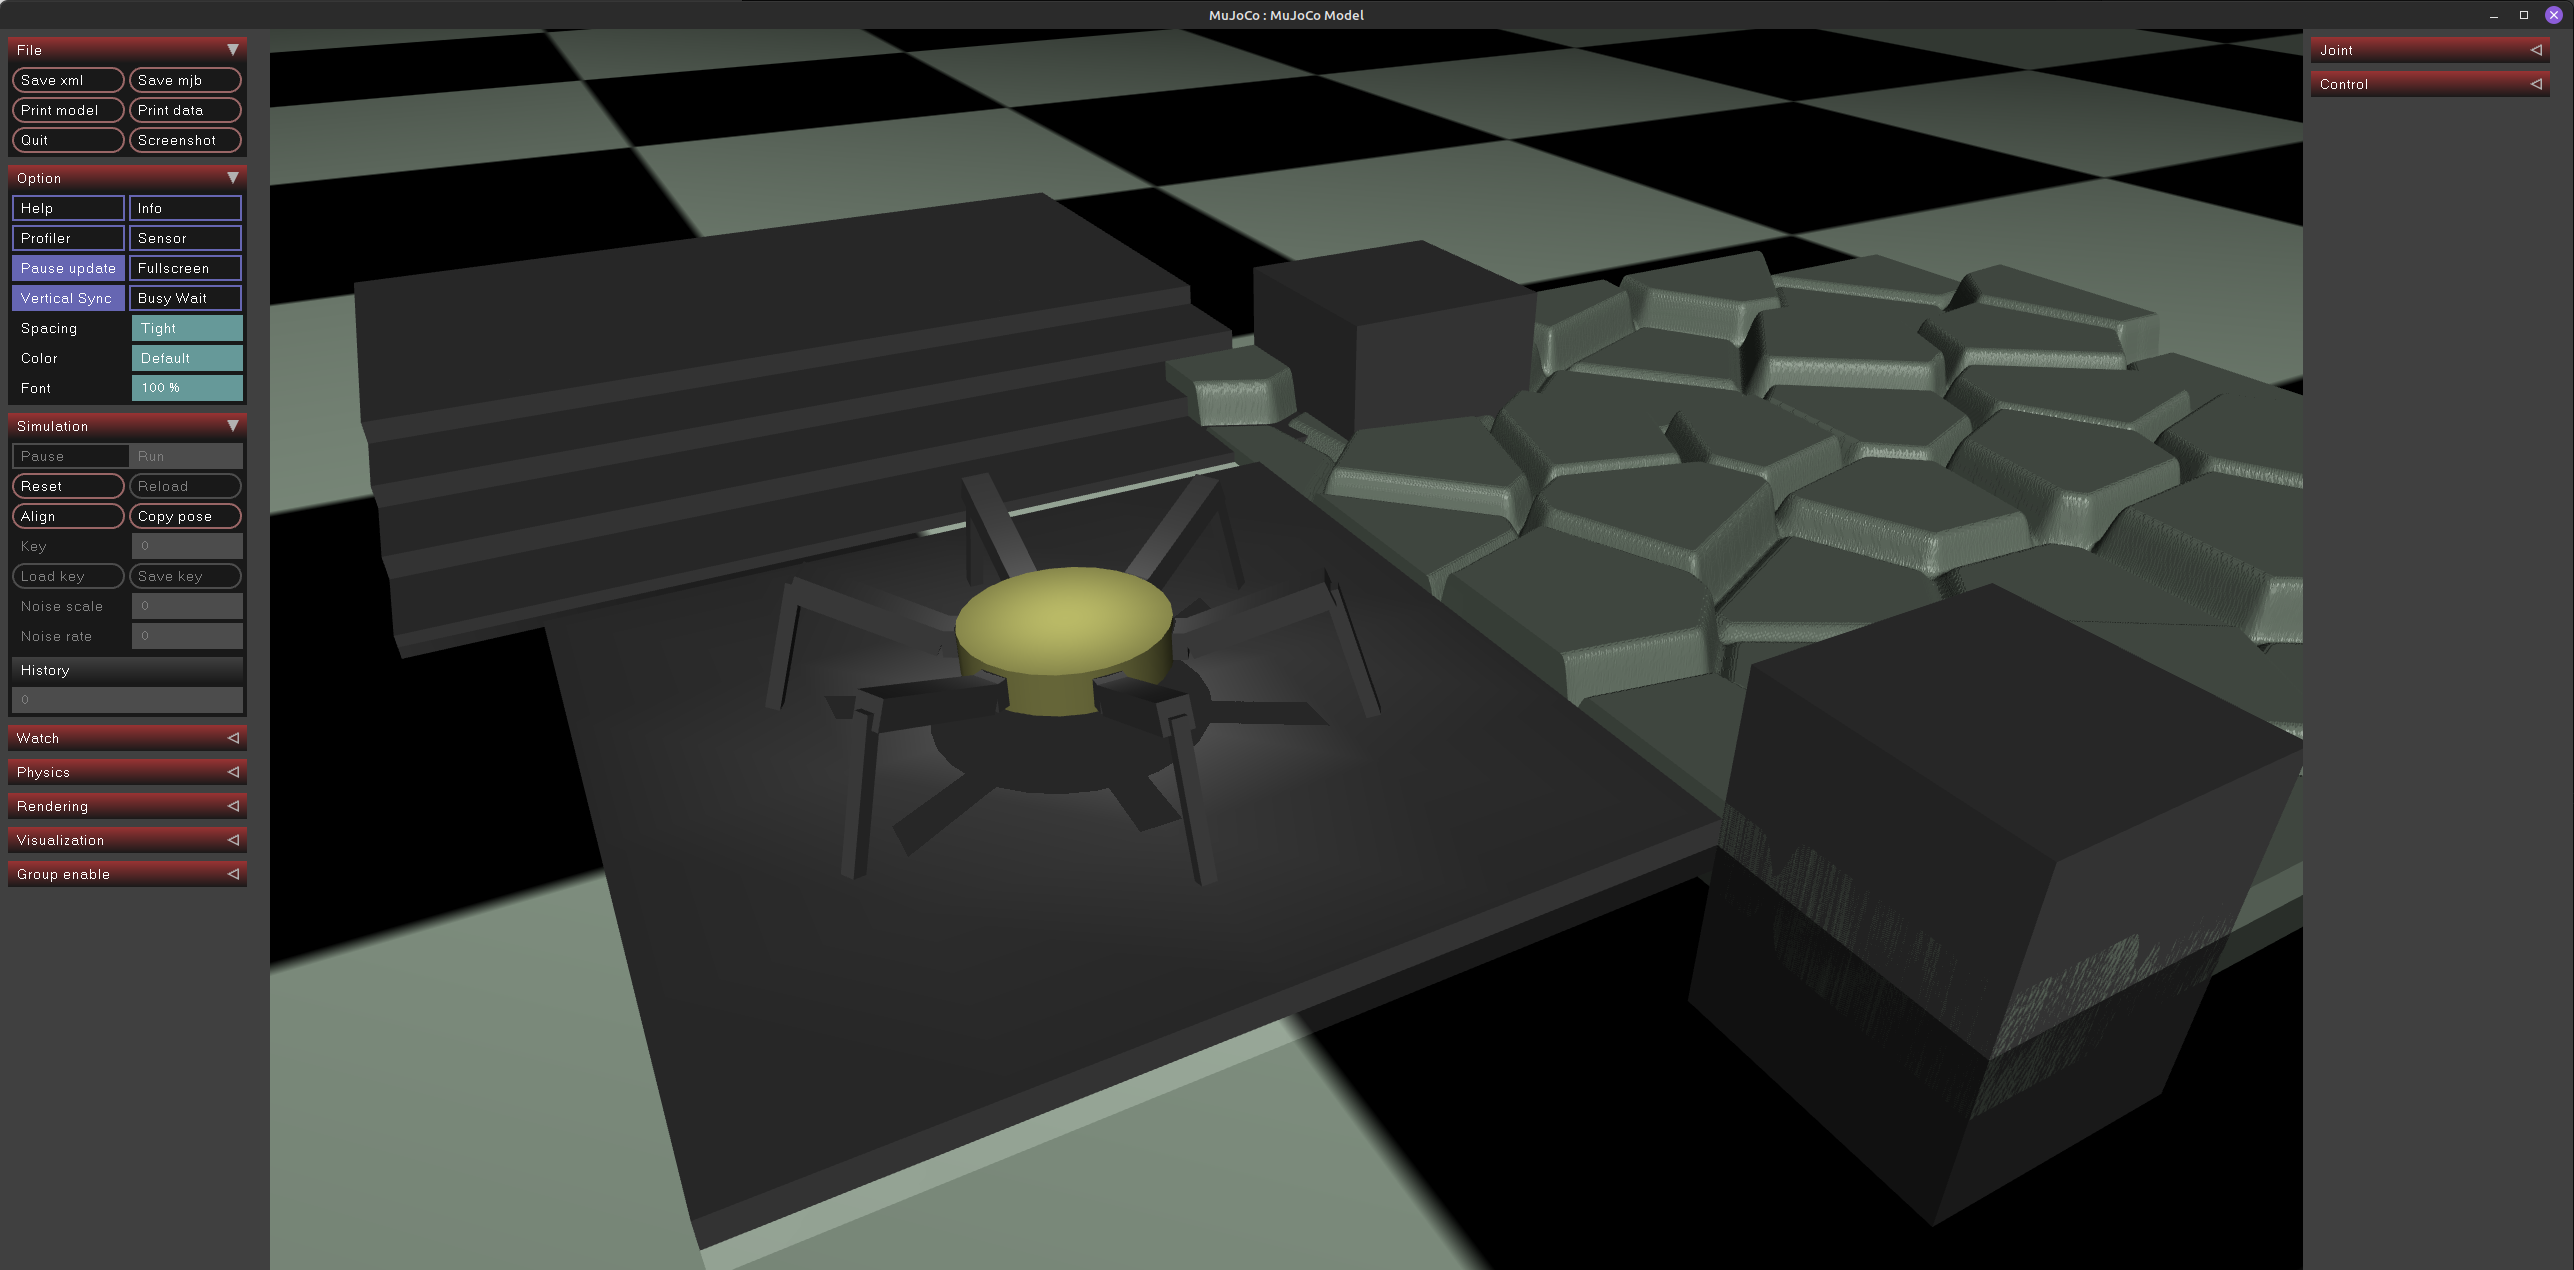
\includegraphics[width=\linewidth]{mujoco.png}
    \caption{The MuJoCo simulation environment}
    \label{fig:mujoco}
\end{figure}

% \bigskip
% \bigskip
% \hrule
% \smallbreak
% \hrule
